\section{The ARGUS Framework}
\label{sec:framework}

\paragraph{Identification rubric.}
ARGUS decomposes a DID study into 11 auditable dimensions (parallel trends, no
anticipation, staggered timing, SUTVA/spillovers, control group, specification,
inference, sample period, concurrent policies, placebo/robustness, data
measurement). Each dimension is an
assumption~$\rightarrow$~implication~$\rightarrow$~evidence chain encoded in
\texttt{config/identification\_dimensions.yaml}.

\paragraph{Bounded-agentic pipeline.}
The audit runs a fixed, deterministic sequence
\emph{decomposition $\rightarrow$ extraction $\rightarrow$ assessment
$\rightarrow$ localization $\rightarrow$ report} (Figure~\ref{fig:arch}, top).
Control flow is code, not a model decision. Agency is confined to
\emph{extraction} and \emph{assessment}, each a bounded ReAct-style loop with
(i)~a small fixed tool set (\texttt{evidence\_search}, \texttt{figure\_parse},
\texttt{policy\_lookup}), (ii)~a hard step budget, and (iii)~a logged trace. This
buys reproducibility and evidence-traceability, which the evaluation
(\S\ref{sec:evaluation}) depends on.

\begin{figure}[t]
  \centering
  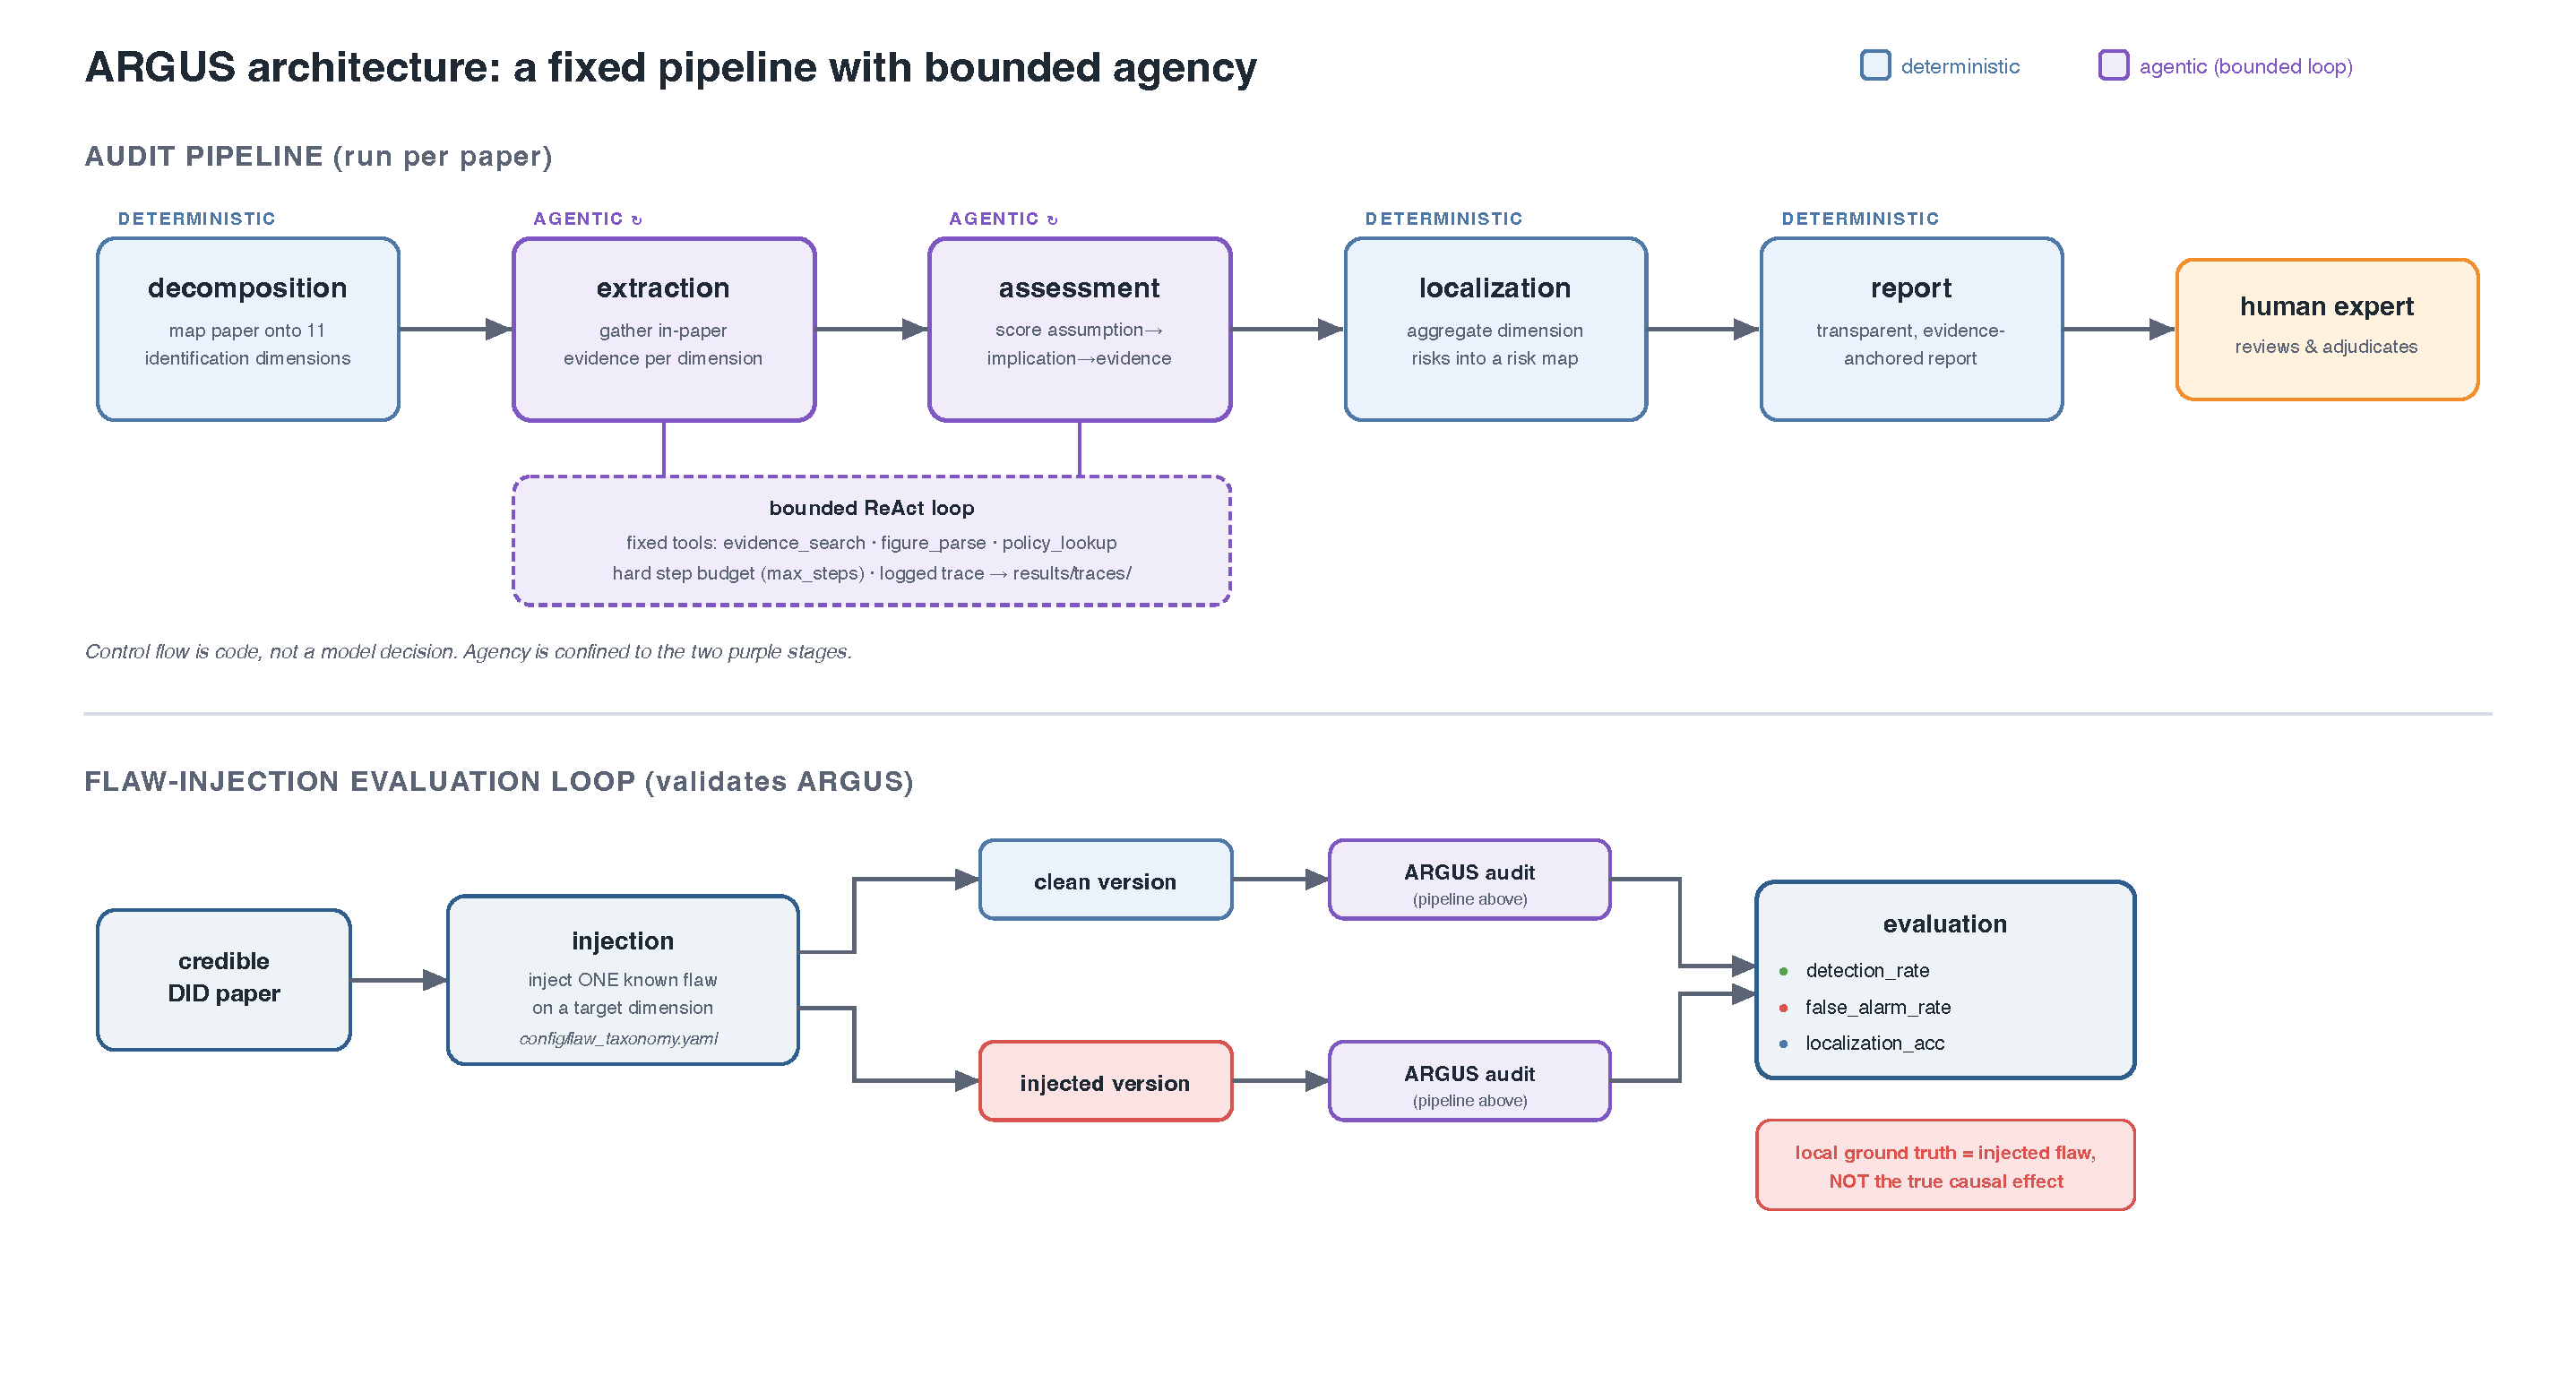
\includegraphics[width=\textwidth]{figures/figure3}
  \caption{ARGUS architecture. \emph{Top:} the audit pipeline is a fixed
  deterministic sequence; agency is confined to the two green stages, each a
  bounded ReAct loop with a fixed tool set, a hard step budget, and a logged
  trace. \emph{Bottom:} the flaw-injection evaluation loop injects one known
  flaw, audits the clean and injected versions, and scores detection,
  false alarm, and localization against the injected flaw as local ground
  truth---never against the unobserved true effect.}
  \label{fig:arch}
\end{figure}

\paragraph{Output.}
ARGUS emits \emph{(study, identification dimension, risk)} triplets with
evidence-grounded rationales for a human expert---never a verdict on the true
causal effect.
